%\documentclass[conference]{IEEEtran}
\documentclass[10pt,onecolumn,letterpaper]{article}
\usepackage{cite}
\usepackage{amsmath,amssymb,amsfonts}
\usepackage{algorithmic}
\usepackage{graphicx}
\usepackage{textcomp}
\usepackage{xcolor}
\usepackage{tabularx,booktabs}
\usepackage[utf8]{vietnam}
\def\BibTeX{{\rm B\kern-.05em{\sc i\kern-.025em b}\kern-.08em
		T\kern-.1667em\lower.7ex\hbox{E}\kern-.125emX}}
\begin{document}
	
	\title{Video Understanding : A review of action detection-recognition dataset}
	%
	%\author{\IEEEauthorblockN{1\textsuperscript{st} Viet Hang Duong}
		%\IEEEauthorblockA{\textit{Dept of Computer Science} \\
			%\textit{University of Information Technology}\\
			%Ho Chi Minh City, Viet Nam \\
			%hangdv@uit.edu.vn}
		%\and
		%\cpvrauthorblockN{2\textsuperscript{nd} Duc Manh Nguyen Dang}
		%\IEEEauthorblockA{\textit{Dept of Computer Science} \\
			%\textit{University of Information Technology}\\
			%Ho Chi Minh City, Viet Nam \\
			%22520847@gm.uit.edu.vn}
		%\and
		%\IEEEauthorblockN{3\textsuperscript{rd} Ngoc Tram Phan Huynh}
		%\IEEEauthorblockA{\textit{Dept of Computer Science} \\
			%\textit{University of Information Technology}\\
			%Ho Chi Minh City, Viet Nam \\
			%22521500@uit.edu.vn}
		%}%
	
	\author{First Author\\
		{\tt\small firstauthor@i1.org}
		% For a paper whose authors are all at the same institution,
		% omit the following lines up until the closing ``}''.
	% Additional authors and addresses can be added with ``\and'',
	% just like the second author.
	% To save space, use either the email address or home page, not both
	\and
	Second Author\\
	{\tt\small secondauthor@i2.org}
}
\maketitle

\begin{abstract}
	In this article, we provide a summary and an overview of the datasets used in
	the task of action detection/recognition. The datasets will be presented in the
	order of their publication time. For each dataset, we sequentially present four
	aspects: the context of its creation, data distribution, explanations of
	annotations, and data collection methods. \\
\end{abstract}

\section{Introduction}
In video understanding tasks, action recognition and detection are prominent and
meaningful due to their practical applications in daily life. Some notable
applications include Surveillance and Security, Human-Computer Interaction,
Sports Analysis, Entertainment and Gaming, among others. Although deep learning
models designed to solve these problems often require significant computational
resources, with the advancement of computer hardware, the deployment in
real-world scenarios while meeting real-time processing speed has become more
feasible over time.

Besides the requirement for significant computational resources, they also
demand a large and sufficiently complex dataset. In addition to serving as
training data, datasets also provide a portion of data specifically for
evaluating models, thereby establishing a common benchmark for comparing
different models. Over the years, new datasets have emerged, either as additions
to existing datasets or as entirely new ones based on different construction
perspectives. This has increased both the diversity and quantity of available
data, but also inadvertently posed challenges in selecting an appropriate
dataset. Evaluating whether a dataset is suitable for a given research problem
is not merely a matter of its scale. Other characteristics must also be
considered, such as the dataset creator's perspective, data collection methods,
sample size, number of classes, level of annotation detail (spatial, temporal,
sound, etc.), popularity within the research community, the baseline for
comparison, and various other factors. Therefore, it is necessary to carefully
examine datasets relevant to the task, gather information, evaluate, and then
compare them to ultimately select the desired dataset for research purposes.
This process typically consumes a significant amount of time and effort. To
address this issue, in this paper, we aim to compile notable datasets in the
fields of action detection and action recognition, listing them chronologically
while providing concise necessary information regarding:

\begin{itemize}
	\item \textit{Context and construction perspective of the dataset}: Since the
	datasets are presented chronologically, this section clarifies the information
	regarding the background and the authors' perspectives on the shortcomings or
	the necessary additions to older datasets.
	\item \textit{Dataset distribution}: Information about the dataset, such as the
	number of data samples, the number of classes, the train-validation splits, and
	any other available details.
	\item \textit{Annotations}: Explanation of the annotations provided in the
	dataset.
	\item \textit{Data collection methods}: We summarize the data collection
	process employed by the respective author groups on that dataset. This allows
	for a more objective assessment of the dataset's reliability and quality based
	on the researcher's perspective.
\end{itemize}

In section II, we will provide a brief overview of the history and context of
the field of artificial intelligence research from its inception to the
emergence of CNN models and their dominance from image task to video task.
Having a general understanding of the history and context will help readers
understand why datasets have their limitations and continue to evolve over the
years.

In section III, we will list the datasets in the order of their publication time
(measured from the time the accompanying paper is published). Each dataset will
include four pieces of information presented in the following order: "Context
and Construction Perspective of the Dataset," "Annotations," "Dataset
Distribution," and "Data Collection Methods." If some information is not
provided by the authors in the original paper, it will be left blank or omitted.
Additionally, if the authors provide any additional information included in the
dataset, we will allocate a separate section below to describe it. The list of
datasets, along with a brief overview of their publication dates and the
mentioned data quantities, can be found in Fig1..

\section{Overview of History}

Although the field of artificial intelligence emerged in the mid-1990s, it took
several decades for significant progress to be made, thanks to the remarkable
advancements in computer hardware - greater computing power and easier
accessibility. As a result, the research community's interest in AI has
significantly increased. AI competitions began to be organized, particularly in
computer vision, attracting numerous research groups. In 2010, the ImageNet
Large Scale Visual Recognition Challenge (ILSVRC) \cite{ILSVRC} was initiated,
aiming to build upon the success of the PASCAL VOC challenge \cite{PASCALVOC} by
evaluating model performance in image recognition tasks.

ILSVRC, upon its initial launch, garnered significant attention and credibility
within the research community due to its unprecedented scale of data: 1.2
million training images and 1,000 object classes. It attracted participation
from top researchers in the field and further solidified its reputation.

\begin{figure} [h]
	\centering
	
	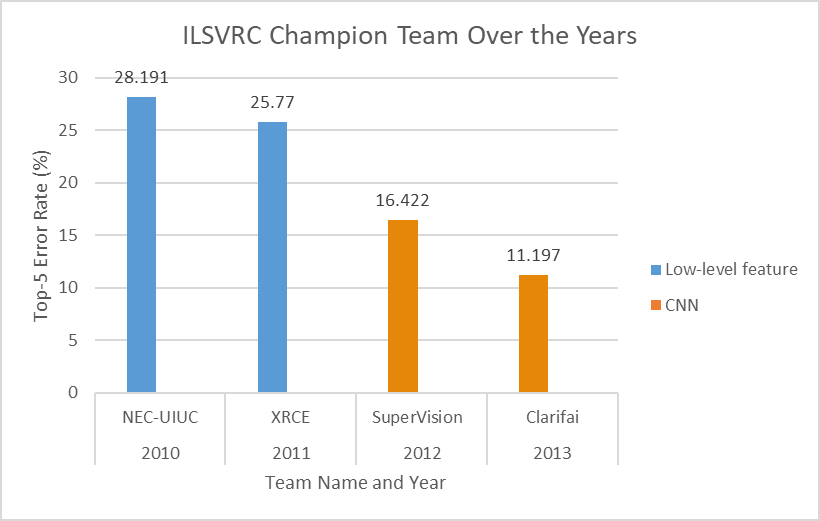
\includegraphics[width=1.\linewidth]{fig_info/fig1/ILSVRCChampionTeamOvertheYears}
	\caption{ILSVRC champion team over years on classification task}
	\label{fig:ilsvrcchampionteamovertheyears}
\end{figure}

Go back to 1998 when LeNet \cite{LeNet}, the first CNN model, was introduced. At
that time, CNN was just one of many research directions and had not received
much attention. It wasn't until 2012 when the SuperVison team, led by
researchers at the University of Toronto, proposed a CNN model called AlexNet
and convincingly won the ILSVRC2012 in image classification with a top-5 error
rate of only 16.422\% (Fig \ref{fig:ilsvrcchampionteamovertheyears}). They
completely outperformed other competitors at that time, paving the way for the
era of CNN and the dawn of Deep Learning. Since then, winning solutions in
subsequent years of ILSVRC have consistently utilized CNN. Over time, there has
been an increasing number of research studies applying CNN models to various
tasks. Through experimentation, CNN has proven to be effective not only in image
classification but also in localization, segmentation, and even beyond computer
vision, extending to other fields such as speech processing and natural language
processing. CNN has shown great potential in developing solutions for previously
challenging problems that were not adequately addressed. One such problem is
action recognition, which is a highly significant task with practical
applications. CNN has opened up possibilities for developing solutions to
previously unresolved problems, and action recognition is just one of them,
receiving considerable attention and practical implications.

The problem of Action Recognition existed before the rise of CNN. Solutions for
action recognition during this period often involved feature extraction using
various methods to obtain a feature vector from the data, followed by a
classifier, typically a Support Vector Machine (SVM). This approach is called
"hand-crafted feature" and it continued to dominate other methods, including
CNNs, until 2015 because CNN models were still relatively new and not
extensively explored. Over time, the research community gradually replaced these
hand-crafted feature methods with CNNs. Continuous advancements and proposals of
CNN models for action recognition have been made, such as Two-stream networks,
Segment-based methods, Multi-stream networks, 3D CNNs, and so on. Alongside
these developments, there has been an increasing demand for computational power
and a significant growth in the amount of data. The datasets used in this period
were also limited, as shown in Table \ref{config}, which lists prominent
datasets from before 2012. It can be observed that in terms of scale (number of
classes, number of video clips), the datasets were still quite limited.

\begin{table}[h]
	\centering
	%\small
	\caption{Action recognition dataset}
	\begin{tabular}{l|l l l l}
		\toprule
		Name & Year & NumClass & Clip/Class & Ref \\
		\midrule
		KTH & 2004 & 6 & 100 & \cite{KTH} \\
		Weizmann & 2005 & 9 & 9 & \cite{Weizmann} \\
		IXMAS & 2007 & 11 & 33 & \cite{IXMAS} \\
		Hollywood & 2008 & 8 & 30-129 & \cite{HollyWood} \\
		UCF Sports & 2008 & 9 & 14-35 & \cite{UCFSports} \\
		Hollywood2 & 2009 & 12 & 61-278 & \cite{Hollywood2} \\
		UCF YouTube & 2009 & 11 & 100 & \cite{UCFYouTube} \\
		Olympic & 2010 & 16 & 50 & \cite{Olympic} \\
		\bottomrule
	\end{tabular}%
	\label{config}
\end{table}%

Building a dataset typically goes through four steps: (1) Defining a set of
predefined actions, (2) Collecting videos from data sources, (3) Annotating the
data (either automatically, semi-automatically, or manually), (4) Cleaning and
filtering the data to remove duplicates and noise. Each step presents its own
challenges. In step (1), defining an action is not a simple task as humans often
perform complex combinations of gestures. So, what constitutes an "atomic
action"? In step (2), do the video sources comply with copyright rules? Privacy
regulations? Is the dataset stable (not prone to loss or replacement)? In step
(3), the workload scales with the dataset size, and there can be vague
boundaries in determining the start and end of an action. In step (4), what
criteria are used to evaluate whether a video meets the standards for usability?
There are many related questions, such as the availability of human and
financial resources, required to meet the demands of building a comprehensive
research dataset. Furthermore, considering the context before CNNs gained
significant prominence, investing in developing a large-scale dataset was highly
risky.

CNN models possess immense power that scales with their complexity., is prone to
overfitting, especially when dealing with small amounts of data. During the
explosion of CNN, research groups faced many challenges due to data scarcity.
Methods like data augmentation were effective solutions, but it was still
necessary to supplement larger and more complex datasets to meet the growing
demand for data in CNN models. Another reason is that the remarkable success of
CNNs in image processing tasks has been greatly contributed by large-scale
datasets like ImageNet. However, in the video domain, there is currently no
comparable dataset to ImageNet. Realizing this need, research groups from all
over the AI research community have continuously improved and published
increasingly refined datasets. These datasets play a crucial role as a common
benchmark for comparing different models.

\section{Review}

\subsection{HMDB51}

\begin{itemize}
	\item Year : 2011
	\item Paper : HMDB: A Large Video Database for Human Motion Recognition
	\cite{HMDB51}.
\end{itemize}

\subsubsection{\textbf{Context and construction perspective}}
KTH \cite{KTH} and Weizmann \cite{Weizmann} have long been regarded as
pioneering datasets in the early stages of action recognition. However, over
time, their limitations have become evident, particularly in terms of a
restricted number of action categories and simplistic background contexts. With
the advent of recent models, achieving accuracy rates exceeding 90\% became
commonplace. As a result, there is a growing demand for alternative datasets
that present more substantial challenges, aiming to push the boundaries and
enhance the capabilities of action recognition systems. The dataset is carefully
designed to highlight differences among action categories based on motion rather
than static poses. With the valuable contribution, the dataset has a potential
of significantly enhance the evaluation and future utilization of recognition
systems in real life. 

\subsubsection{\textbf{Data collection methods}}
A group of student is asked to collect and annotate any segment which represents
a single non-ambiguous human action from videos. The videos are sourced from
digitized movies, public databases like the Prelinger archive, additional online
videos, as well as content from YouTube, Google videos and other videos from
internet. Students also were asked to consider some minimum quality standard : 
only one action per clip, minimum height for main actor should be 60 pixels,
minimum contrast level, minimum of clip length is 1 second, acceptable
compression artifacts, etc. 

\subsubsection{\textbf{Data distribution}} 
It includes 6,766 video clips covering 51 different action categories, with each
category having at least 101 clips. 
\begin{itemize}
	\item Train : for each action, 70 random clips are used.
	\item Validation : no validation set.
	\item Test : for each action, 30 random clips are used. 
\end{itemize}

The authors generated three distinct training/testing split follow above rule,
ensure that no test clip also train clip.

\subsubsection{\textbf{Annotations}}

\begin{figure}[h]
	\centering
	\includegraphics[width=1.\linewidth]{"fig_info/fig2/Untitled Diagram.drawio"}
	\caption{}
	\label{fig:untitled-diagram}
\end{figure}

For each class, there will be 3 split files as mentioned above. Each file will
include the names of all the videos in the same class along with an index
belonging to $\lbrace 0, 1, 2 \rbrace$ as shown in Figure
\ref{fig:untitled-diagram}. The file used for training is indexed as 1, for
testing it is 2, and 0 indicates that it is not used in this split.

\begin{table}[h]
	\centering
	\caption{Action recognition dataset}
	\begin{tabular}{l | l     }
		\toprule
		PROPERTY & CATEGORIES \\
		\midrule
		Visible body parts & head(h), upper body(u), full body (f), lower body(l)\\ 
		Camera motion & motion (cm), static (nm) \\
		Number of people involved in the action	& single (np1), two (np2), three
		(np3)\\
		Camera viewpoint & front (fr), back (ba), left(le), right(ri) \\
		Video quality & good (goo), medium (med), ok (bad)	\\
		
		
		\bottomrule
	\end{tabular}%
	\label{config2}
\end{table}%

The name of each video also carries a meaning, with a specific structure as
follows: \\
\text{vid-name\_class-name\_vible-body-part\_cam-motion\_num-of-people\_cam-viewpoint\_vid-quality}\\
The abbreviations used are listed in Table \ref{config2}. \\
For example, the name
IPL\_Awards\_Ceremony\_shake\_hands\_f\_cm\_np2\_ba\_med\_0.avi represents a
video titled IPL Awards Ceremony, belonging to the shake hands class, with 'f'
indicating full body, 'cm' indicating motion, 'np2' indicating two people, 'ba'
representing back viewpoint, and 'med' indicating medium quality.
\subsection{Something Something V2}

\begin{itemize}
	\item Year : 2017
	\item Paper : The “something something” video database for learning and evaluating visual common sense
	Actions \cite{somethingsomething}
\end{itemize}

\subsubsection{\textbf{Context and construction perspective}}

The recent expansion of the Action Recognition dataset has led to a rapid increase in the number of videos available, particularly sourced from platforms like YouTube such as Sport-1M \cite{Sports1M} and Youtube-8M \cite{YouTube8M}. However, the model's work associated with these datasets still involves combining features extracted from frames, and therefore becoming a "set of image" classification task. That's the reason even these datasets empower models to infer numerous actions depicted in videos, they often lack the contextual understanding of how different actions correlate with each other. Consequently, when an action is combined with various objects, it can potentially mislead the model since it diverges from its learned associations. As an illustration, consider the action of "pointing to," which can result in two scenarios: "Pointing a finger" (Harmless) or "Pointing a knife to" (Dangerous). The objective of Something Something dataset is to address this particular problem.

In the related paper \cite{somethingsomething}, Something V1 emphasizes detailed interactions between human actions and objects, aiming to provide fine-grained videos that reflect real-world aspects. Later, the V2 version was released and significantly increasing the number of videos and improving label quality.
\subsubsection{Data collection methods}
A group of workers from the crowdsourcing service Amazon Mechanical Turk (AMT) were asked to record and label clips. They recorded videos that demonstrated specific actions with the given labels. After the video is uploaded, it is divided into categories depends on its action, label, and object information. Afterward, they submitted the videos to an online platform, which underwent careful automatic quality checks. Each submission was then rechecked by other workers to make sure there is no mistaken.
\subsubsection{Data distribution}
In the newer V2 version, the number of videos has increased to 220,847 clips, which is twice the number in V1, while retaining the same set of labels totaling 174. Overall, there are 318,572 annotations, which involve 30,408 unique objects. The data is split into training, validation, and test sets with a ratio of 8:1:1. Additionally, measures are taken to ensure that videos created by a single actor are exclusively allocated to one of these three splits. 
\begin{itemize}
	\item Train : 168,913 clips
	\item Validation : 24,777 clips
	\item Test: 27,157 clips
\end{itemize}
\subsubsection{Annotation}

An interesting aspect of this dataset is its provision of "sentence-like" information alongside the focus on human actions. This augmentation allows for descriptions of how actors interact with objects. For instance, a video featuring the phrasal verb's action "moving away" might be presented as: "Moving a bag of popcorn away from the camera". By integrating object names with actions, the dataset offers detailed action descriptions. 

Due to the unique labeling approach using "natural language," conventional one-hot encoding methods are not applicable. Consequently, it is recommended that model should be first pretrain on ImageNet to enhance the capture of distinctive object characteristics.

For videos in the training set marked by a unique ID, there is an annotated JSON file records detailed descriptions which includes Video IDs (containing only the training video's ID), completed labels (providing precise descriptions of the actor's actions), template categories (outlining the action skeleton), and placeholders (identifying objects used in the video).

For example: {"id":"217769","label":"moving a bag of popcorn away from the camera","template":"Moving [something] away from the camera","placeholders":["a bag of popcorn"]}
\subsection{AVA}

\begin{itemize}
	\item Year : 2018
	\item Paper : AVA: A Video Dataset of Spatio-temporally Localized Atomic Visual
	Actions \cite{AVA}
\end{itemize}

\subsubsection{\textbf{Context and construction perspective}}

Popular action classification datasets such as KTH \cite{KTH}, Weizmann
\cite{Weizmann}, HMDB51 \cite{HMDB51}, and UCF101 \cite{UCF101} only consist of
short clips manually trimmed to capture a single action. Newer datasets like
Sports-1M \cite{Sports1M}, YouTube-8M \cite{YouTube8M}, Something-something
\cite{somethingsomething}, and Moments in Time \cite{momentsintime} focus on
larger-scale data and are often annotated automatically, leading to noisy
annotations. Some recent studies, such as ActivityNet \cite{ActivityNet}, THUMOS
\cite{THUMOS}, and Charades \cite{Charades}, utilize a large number of videos
containing multiple actions but only provide temporal annotations. Recognizing
the limitations from their perspective, the authors of this paper proposed the
AVA dataset.

\subsubsection{Data collection methods}

The process of constructing the AVA dataset involves five steps : action
vocabulary generation, movie and segment selection, person bounding box
annotation, person linking and action annotation.

\begin{itemize}
	\item \textbf{Action vocabulary generation} : They generate action vocabulary
	base on three principle :  
	\subitem \textit{Generality} : Generic action in daily-life scenes, opposite of
	specific actions in a specific situation, for example, playing football on a
	football field, would be general or nonspecific actions in a general situation.
	\subitem \textit{Atomicity} : Independent of interacted objects (e.g., hold
	without specifying what object to hold).
	\subitem \textit{Exhaustivity} : The authors initialized list of actions using
	knowledge
	from previous datasets. They iterated through this list multiple times until it
	covered approximately 99\% of the actions in the AVA dataset.
	
	\item \textbf{Movie and segment selection} : Raw video content is sourced from YouTube. The authors initially compile a list of top actors from various nationalities. Each actor is then searched using a YouTube query, retrieving up to 2000 results. The selected videos must fall under the categories of "film" or "television," have a duration of over 30 minutes, be uploaded at least one year prior, and have a minimum of 1000 views. Additionally, black and white videos, low-resolution videos, animated and cartoon content, gaming videos, as well as videos containing adult content, are excluded. Each video is partition into a 15-minute long segment and divided into 897 movie segments. The result is 430 videos.
	
	\item \textbf{Person bounding box annotation} : First, the bounding boxes are automatically detected using the Faster-RCNN \cite{faster-rcnn} person detector, which significantly reduces the manual annotation time. Then, annotators re-annotate the missed boxes to ensure complete coverage. In the final step, incorrectly labeled boxes are marked and removed.
	
	\item \textbf{Person link annotation} : The bounding boxes are linked using person embeddings \cite{personembedding}, and then the optimal matching with the Hungarian algorithm \cite{TheHungarian} is applied to match the boxes together. In order to increase accuracy, annotators remove false positive boxes in the next step.
	
	\item \textbf{Action annotation} : Recognizing the practicality that annotators may make labeling mistakes is unavoidable when dealing with up to 80 classes, the authors divided Action annotation into two stages: action proposal and verification. In the proposal stage, annotators are required to suggest action classes, and these proposals are verified by annotators in the verification stage.
	
\end{itemize}
	
\subsubsection{Data distribution}
	
	In total, there are 430 videos covering 80 classes, with each video contributing 15 minutes at a sample rate of 1Hz (meaning one frame per second, 897 segments per 15 minutes). The train/val/test ratio is divided as 55:15:30, respectively.
	\begin{itemize}
		\item Train : 235 videos, 211k segments.
		\item Val : 64 videos, 57k segments.
		\item Test : 131 videos, 118k segments.
	\end{itemize}
	
\subsubsection{Annotation}

The AVA action dataset has four versions : v1.0, v2.0, v2.1 and v2.2. There are two key differences between AVA v2.2 and v2.1. Firstly, an additional round of human rating was carried out to include missing labels, resulting in a 2.5\% increase in the total number of annotations. Secondly, box locations were corrected for a few videos that had aspect ratios significantly larger than 16:9. Regarding AVA v2.1, the only modification compared to v2.0 was the removal of a few duplicate movies. The class list and label map remained unchanged from v1.0. The differences between v1.0 and v2.0 is not mentioned by authors.

\begin{figure}[h]
	\centering
	\includegraphics[width=0.7\linewidth]{"fig_info/fig3/Untitled Diagram.drawio"}
	\caption{}
	\label{fig:untitled-diagram2}
\end{figure}

Figure \ref{fig:untitled-diagram2} lists the annotation files provided across different versions, v2.0 is not mentioned because it has been replaced by v2.1. Unlike v1.0, v2.1, and v2.2 include additional action list files (60 classes as a subset of the 80 classes in AVA), which serve the purpose of the ActivityNet Challenge \cite{ActivityNet}. Additionally, there are included files and excluded files. Raters typically provided annotations at timestamps ranging from 902 to 1798, inclusive, in seconds, with a 1-second interval. Performance evaluation includes all these "included" timestamps, even those where raters indicated the absence of any action. However, for certain videos, specific timestamps were excluded from annotation due to raters flagging the corresponding video clips as inappropriate. Evaluation of performance does not take into account the "excluded" timestamps.\\

The format of a row is the following: video\_id, middle\_frame\_timestamp, person\_box, action\_id, person\_id , as described on the official website :
\begin{itemize}
	\item video\_id: YouTube identifier
	\item middle\_frame\_timestamp: the timestamp in seconds from the start of the YouTube video
	\item person\_box: the bounding box coordinates of the person, given as the top-left $(x_1, y_1)$ and bottom-right $(x_2, y_2)$ points normalized with respect to the frame size. The coordinate range is from $(0.0, 0.0)$ at the top left to $(1.0, 1.0)$ at the bottom right.
	\item action\_id: the identifier of an action class
	\item person\_id: a unique integer that allows linking this box to other boxes depicting the same person in adjacent frames of the video.
\end{itemize}

\bibliographystyle{ieeetr}
\bibliography{references.bib}

\end{document}


s